\chapter{Codebase: The core}

The first part of the codebase that one would want to look at is the
core.  This is located at ./src/core.  Code contained in this
directory initializes the WDAT object and provides the utiilities and
major components that will be utilized through out the lifetime of
WDAT in the browser memory.


\section{core.js}

Defines the 'wdat' object as a global property of the window object.
This allows one to refer to the 'wdat' object as simply wdat from
within any scope.

\section{config.js}

Defines the 'wdat.v' object which contains values that will be used
throughout the application.  It provides a singular point of entry for
all the configuration directives for this application.

\subsection{Notable directives}

\begin{description}
  \item[wdat.v.l]\hfill \\
  contains layout dimensions, fractions and page width/height.

  \item[wdat.v.u]\hfill \\
  contains url resource endpoints for login, logout etc.

  \item[wdat.v.m]\hfill \\
  contains miscellaneous directives.
\end{description}

\section{bootstrap.js}

Defines a wdat.init() function and calls it.

wdat.init creates the primary divisions to introduce widgets into. It
also introduces some functions that should be a part of the javascript
library but aren't.  These functions are for primary string operations
or for type-checking.

\begin{figure}[h!t]
  \centering
  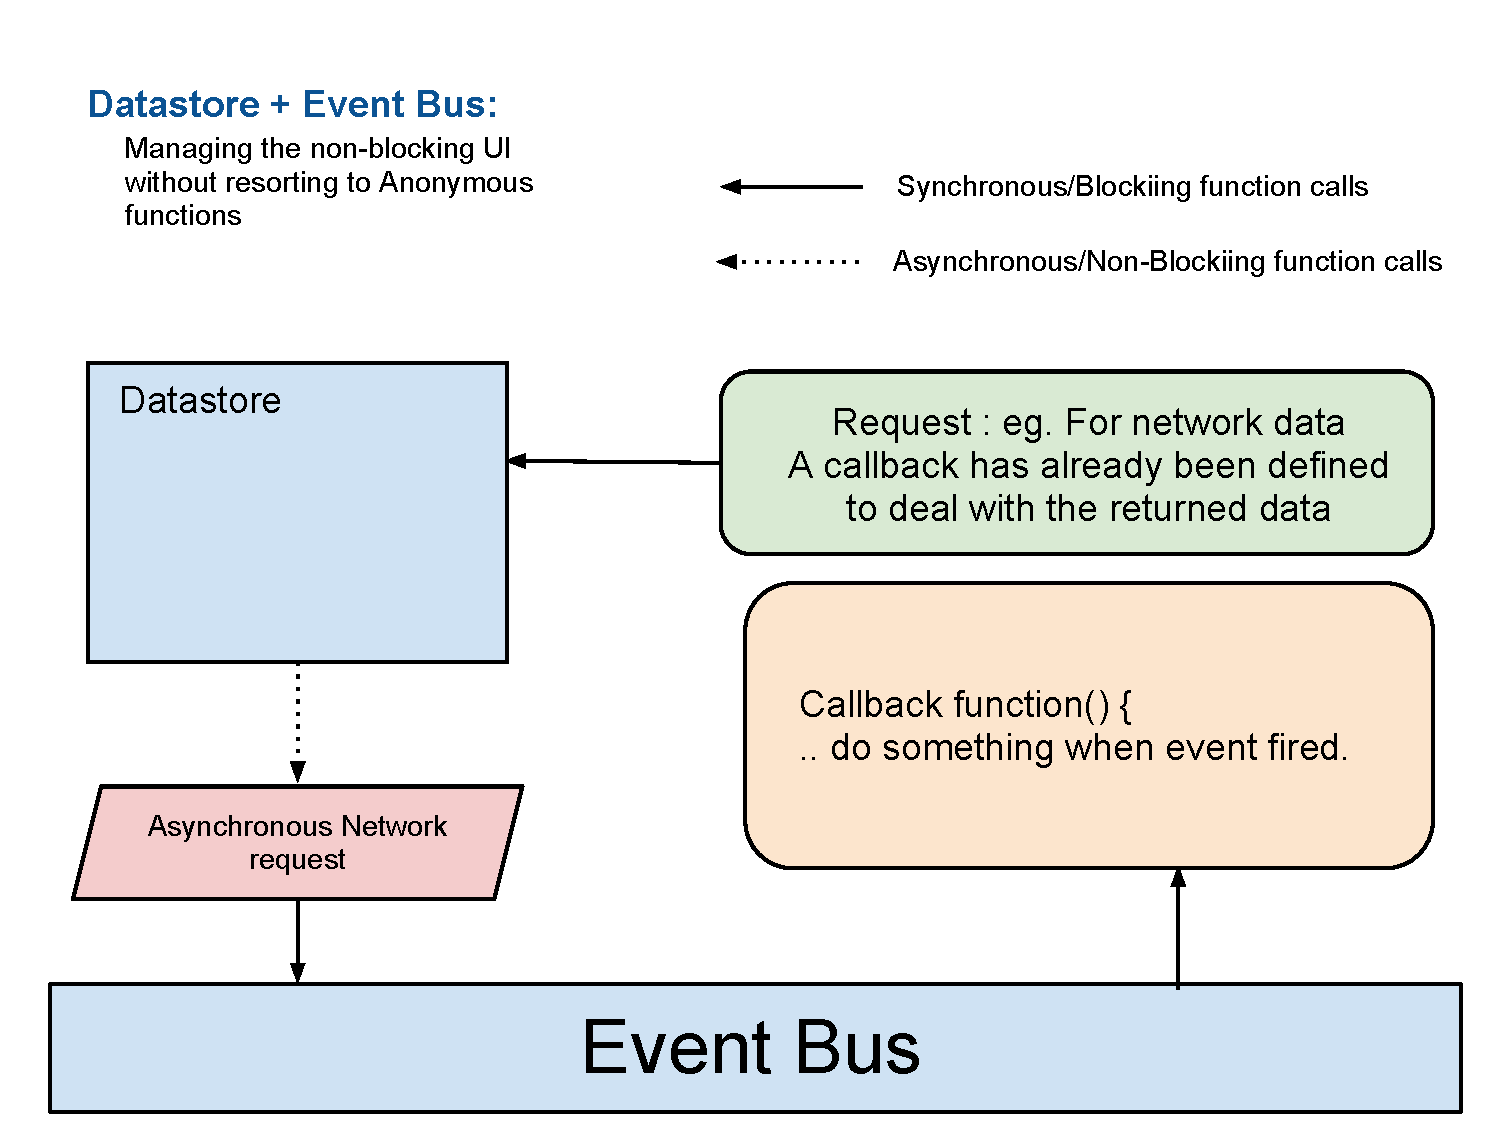
\includegraphics[width=\textwidth]{src/images/DatastoreAndEventBus.pdf}
  \caption{How the event bus is used for making asynchronous network requests without hurting readability and modularity of the code.}
\end{figure}

\section{datastore.js}

The datastore is an integral part of the wdat application.  It is an
abstraction layer for fetching data from the servers and also does
some trivial caching in the realm of the application.  

The datastore exposes common methods to access metadata objects, data
objects and datafiles.  

Network connectivity in a browser environment is best managed
asynchronously.  To implement the datastore in an async manner without
making use of nested anonymous functions, some pretty interesting
patterns are used.

When the calling program requests some data to be downloaded, it also
provides a unique id to the request, say uid.  Now this is a
non-blocking call and the program proceeds without the UI hanging.
When the request has been completed and the object received from the
servers, it is parsed into a javascript object and an event
'ReceivedData\textunderscore\textless\textless<uid>>\textgreater\textgreater'
is fired with this javascript object being appended to the event as a
parameter.

Any functions that are subscribed to this event are notified and they
begin executing upon this particular data.

Note: caching is already provided by the browser but that is still on
a network connectivity level.

\section{eventBus.js}

The event bus is one of the most important parts of the application.
Even though it is hardly 20 lines of code, it is integral to the
inherent asynchronous nature of the application.

The EventBus exposes two functions.  wdat.bus.publish() and
wdat.bus.subscribe():

\begin{description}
  \item[subscribe()] \hfill \\
  allows you to setup a callback function to be called,
  albeit, asynchronously when some event is fired.

  \item[publish()] \hfill \\
  allows one to fire a event along with a set of parameters.
  Once a publish() is done, all subscriptions to this particular event
  are called with parameters (if any) supplied as arguments to the
  function. 
\end{description}

All data updates and notifications are done through the EventBus.


As shown in figure 3.1, the event bus is central to asynchronousness in
the application.

\section{uid.js}

UID are unique numeric strings used throughout WDAT to uniquely
identify events.  wdat.uid() is the only defined function in this
module.  Calling wdat.uid() multiple times returns unique numeric
strings each time.

